%~~~~~~~~~~~~~~~~~~~~~~~~~~~~~~~~~~~~~~~~~~~~~~~~~~~~~~~~~~~~~~~~~~~~~~~~~~~~~~~~~~~~~~~~~%
% IISER Thiruvananthapuram Presentation/Beamer Format
% LaTeX Template
%
% Copyright (c) 2022 by Nikhil Alex Verghese, BS-MS '17, IISER Thiruvananthapuram
%
% This work is licensed under the Creative Commons Attribution 4.0 International License.
% (CC BY-NC-SA 4.0)
%
% To view a copy of this license, visit ``http://creativecommons.org/licenses/by-nc-sa/4.0/'' or send a letter to Creative Commons, PO Box 1866, Mountain View, CA 94042, USA.
%
% FORWARD ANY AND ALL SUGGESTIONS TO: nikhil.alexv17@alumni.iisertvm.ac.in
%
% READ ALL INSTRUCTIONS (presented as comments) IN EACH TEX FILE CAREFULLY.
%~~~~~~~~~~~~~~~~~~~~~~~~~~~~~~~~~~~~~~~~~~~~~~~~~~~~~~~~~~~~~~~~~~~~~~~~~~~~~~~~~~~~~~~~~%

% Comments like this begin with a % character.
% Ctrl+b for \textbf{bold} and Ctrl+i for \textit{italics}

% Refer to these links for useful beamer tips and tricks
% http://tug.ctan.org/macros/latex/contrib/beamer/doc/beameruserguide.pdf
% https://www.overleaf.com/learn/latex/Beamer
% https://en.wikipedia.org/wiki/Beamer_%28LaTeX%29 --> `External Links'

% THE FOLLOWING TEMPLATE IS FRAGILE:
% It is recommended you familiarise yourself with a rough idea of the presentation's framework before adding custom elements.

% THE FOLLOWING TEMPLATE DOES NOT SUPPORT THE USE OF FRAME SUBTITLES.

%~~~~~~~~~~~~~~~~~~~~~~~~~~~~~~~~~~~~~~~~~~~~~~~~~~~~~~~~~~~~~~~~~~~~~~~~~~~~~~~~~~~~~~~~~%
%	                  PREAMBLE (PACKAGES AND DOCUMENT CONFIGURATION)                      %
%~~~~~~~~~~~~~~~~~~~~~~~~~~~~~~~~~~~~~~~~~~~~~~~~~~~~~~~~~~~~~~~~~~~~~~~~~~~~~~~~~~~~~~~~~%

\documentclass[10pt,presentation,shownotes,aspectratio=169]{beamer}
\usetheme{Warsaw} % Use of other themes is not highly recommended as its features would clash with other custom-defined ones.
\usecolortheme{crane} % Yellow colour scheme, others include default, beaver, dolphin, dove, lily, orchird, rose, seahorse, wolverine and whale.
\usefonttheme{default}
\setbeamertemplate{caption}[numbered]
\setbeamercolor{block body example}{bg=green!12}
%\setbeamertemplate{navigation symbols}{} % Uncomment to disable the bottom right navigation buttons
%\setbeamercovered{transparent}
\setbeamertemplate{theorems}[numbered]

\usepackage[utf8]{inputenc}
\usepackage[T1]{fontenc}
\usepackage{lmodern}
\usepackage[english]{babel}
\usepackage{csquotes}
\usepackage{mathtools,amsfonts,amssymb,setspace}

\usepackage{pstricks} % PSTricks offers an extensive collection of quick and easy macros for generating PostScript including macros for colour, graphics, pie charts, rotation, trees and overlays. 
% (https://ctan.org/pkg/pstricks-base?lang=en)

\usepackage{hyperref} % hyperref package for creating reliable hyperlinks and customizations
% (https://ctan.org/pkg/hypperref?lang=en)

\usepackage{tikz} % Tikz package for drawing graphs and diagrams [XY-pic is now outdated]
% (https://ctan.org/pkg/tikz?lang=en, https://www.overleaf.com/learn/latex/TikZ_package)

%\usepackage{tikz-cd} % Commutative Diagrams with Tikz, primarily for linear algebra.
% (https://ctan.org/pkg/tikz-cd?lang=en)

%\usepackage{pgfplots} % The Pgfplots package is dependent on tikz package and is used to portray detailed 2D and 3D function plots from scratch as well as plot available data with a high degree of customization (https://www.overleaf.com/learn/latex/Pgfplots_package) 
% (https://ctan.org/pkg/pgfplots?lang=en)

%\usepackage{caption} % The captions package allows you to better control captions for floating environments like figures, etc. 
% (https://ctan.org/pkg/caption?lang=en)

%\usepackage{booktabs} % The booktabs package allows better control over tables including ruling, width, etc. (https://ctan.org/pkg/booktabs?lang=en) 

\usepackage{xcolor} % Customize colours for hyperlinks, etc.
% (https://ctan.org/pkg/xcolor?lang=en)
\hypersetup{
	colorlinks,
	linkcolor={blue!50!black},
	citecolor={blue!50!black},
	urlcolor={blue!80!black}
}

\usepackage[toc,page]{appendix}
%\usepackage{appendixnumberbeamer} % This resets the page count after the \appendix function is called, unlike the traditional appendix package 
% (https://ctan.org/pkg/appendixnumberbeamer?lang=en)

\usepackage[backend=biber,style=alphabetic]{biblatex} % We use BiBLaTeX for our bibliography.
% (https://ctan.org/pkg/biblatex?lang=en)
\renewcommand*{\nameyeardelim}{\addcomma\addspace}
\addbibresource{ref.bib}

\usepackage{lipsum} % The lipsum package is for generating dummy text throughout this template and is not necessary.

% \usepackage{verbatim} % The verbatim package is useful upon needing to display large amounts of code as is.

%\usepackage{siunitx} % The siunitx package helps typeset units of all kinds. 
% (https://ctan.org/pkg/siunitx?lang=en)

%\usepackage{chemformula} % The chemformula package is a must for typesetting chemical compounds and reactions.

%~~~~~~~~~~~~~~~~~~~~~~~~~~~~~~~~~~~~~~~~~~~~~~~~~~~~~~~~~~~~~~~~~~~~~~~~~~~~~~~~~~~~~~~~~%

% Note: Changes to specific presentation elements usually start with /makeatletter and end with /makeatother in a tex file.

% Defining our Remark Block
\makeatletter
\def\th@remark{%
    \normalfont % body font
    \setbeamercolor{block title example}{bg=orange,fg=black}
    \setbeamercolor{block body example}{bg=orange!20,fg=black}
    \def\inserttheoremblockenv{exampleblock}
  }
\makeatother

\theoremstyle{remark}
\newtheorem*{remark}{Remark}

% Defining Corollary Block
\makeatletter
\def\th@corollary{%
    \textit % body font
    \setbeamercolor{block title example}{bg=blue,fg=black}
    \setbeamercolor{block body example}{bg=blue!20,fg=black}
    \def\inserttheoremblockenv{exampleblock}
  }
\makeatother

% Setting Header Properties
\setbeamertemplate{headline}
{
  \leavevmode%
  \hbox{%
  \begin{beamercolorbox}[wd=.5\paperwidth,ht=2.5ex,dp=1ex,left,leftskip=1em]{section in head/foot}%
    \usebeamerfont{subsection in head/foot}\hspace*{2ex}\insertshorttitle
  \end{beamercolorbox}%
  \begin{beamercolorbox}[wd=.5\paperwidth,ht=2.5ex,dp=1ex,center]{date in head/foot}%
    \usebeamerfont{date in head/foot}\insertshortdate{}\hspace*{2ex}
  \end{beamercolorbox}}%
  \vskip0pt%
}

% Defining the Title Page, you can comment/remove all of the following lines to return it to default (all centered).
\makeatletter
\defbeamertemplate*{title page}{mytitlepage}[1][]
{
  \vbox{}
  \vfill
  \begingroup
    \centering
    \parbox{.75\paperwidth}{% change the width here
    \begin{beamercolorbox}[wd=\linewidth,sep=8pt,center,#1]{title}
      \usebeamerfont{title}\inserttitle\par%
      \ifx\insertsubtitle\@empty%
      \else%
        \vskip0.25em%
        {\usebeamerfont{subtitle}\usebeamercolor[fg]{subtitle}\insertsubtitle\par}%
      \fi%     
    \end{beamercolorbox}%
    }
    \vskip1.3em
  \endgroup
  \begingroup
        \begin{beamercolorbox}[sep=8pt,left,#1]{author}
        \usebeamerfont{author}\insertauthor
        \end{beamercolorbox}
        \begin{beamercolorbox}[sep=8pt,left,#1]{institute}
        \usebeamerfont{institute}\insertinstitute
        \end{beamercolorbox}
        \begin{beamercolorbox}[sep=8pt,left,#1]{date}
        \usebeamerfont{date}\insertdate
        \end{beamercolorbox}
   \endgroup
        \vskip-7.5em
        \hfill
        {\usebeamercolor[fg]{titlegraphic}\inserttitlegraphic\par}
        \vspace{0pt plus 0.4fill} 
}
\setbeamertemplate{title page}[mytitlepage][colsep=-4bp,rounded=true,shadow=\beamer@themerounded@shadow]
\makeatother

% Setting Footer Properties
\makeatletter
\setbeamertemplate{footline}
{
  \leavevmode%
  \hbox{%
  \begin{beamercolorbox}[wd=.33\paperwidth,ht=2.25ex,dp=1ex,center]{author in head/foot}%
    \usebeamerfont{author in head/foot}\insertshortauthor~~\beamer@ifempty{\insertshortinstitute}{}{(\insertshortinstitute)}
  \end{beamercolorbox}%
  \begin{beamercolorbox}[wd=.34\paperwidth,ht=2.25ex,dp=1ex,center]{subsection in head/foot}%
    \usebeamerfont{section in head/foot}\hspace*{1ex}\insertsectionhead\hspace*{1ex}
  \end{beamercolorbox}%
  \begin{beamercolorbox}[wd=.33\paperwidth,ht=2.25ex,dp=1ex,right, rightskip=1em]{section in head/foot}%
    \usebeamerfont{section in head/foot}\insertsubsectionhead\hspace*{2ex}
  \end{beamercolorbox}}%
  \vskip0pt%
}
\makeatother

% Defining when a title is required for a frame
\makeatletter
\setbeamertemplate{frametitle}{
    \ifbeamercolorempty[bg]{frametitle}{}{\nointerlineskip}%
    \@tempdima=\textwidth%
    \advance\@tempdima by\beamer@leftmargin%
    \advance\@tempdima by\beamer@rightmargin%
    \begin{beamercolorbox}[sep=0.3cm,center,wd=\the\@tempdima]{frametitle}
        \usebeamerfont{frametitle}%
        \vbox{}\vskip-1ex%
        \if@tempswa\else\csname beamer@ftecenter\endcsname\fi%
        \strut\insertframetitle\strut\par%
        {%
            \ifx\insertframesubtitle\@empty%
            \else%
            {\usebeamerfont{framesubtitle}\usebeamercolor[fg]{framesubtitle}\insertframesubtitle\strut\par}%
            \fi
        }%
        \vskip-1ex%
        \if@tempswa\else\vskip-.3cm\fi% set inside beamercolorbox...
    \end{beamercolorbox}%
}
\makeatother


% Setting a self-updating ToC at the beginning of every section.
\AtBeginSection[]
{
	\begin{frame}
	\frametitle{Table of Contents}
	\tableofcontents[currentsection]
	\end{frame}
}

% Setting Subsections with their own Frame Titles
\makeatletter
\newcommand<>{\insertsubsectiontitle}{\frametitle{\insertsubsection}}
\let\oldbeamer@checkframetitle\beamer@checkframetitle% Store the \frametitle checking mechanism
\renewcommand<>{\subsection}{%
  \gdef\beamer@checkframetitle{% Update \frametitle checking to ...
    \insertsubsectiontitle% ...insert the section title and...
    \global\let\beamer@checkframetitle\oldbeamer@checkframetitle% ...revert to it's old definition
  }% Regular \section stuff follows
  \alt#1{\@ifnextchar[\beamer@subsection\beamer@@subsection}
    {\beamer@secgobble}}
\makeatother

% Defining proofs environment for proofs requiring more than one frame
\makeatletter
\newenvironment<>{proofs}[1][\proofname]{%
    \par
    \def\insertproofname{#1\@addpunct{.}}
    \usebeamertemplate{proof begin}#2}%
  {\usebeamertemplate{proof end}}
\makeatother

% Uncomment for some standard math notations
% \newcommand{\reals}{\mathbb{R}}
% \newcommand{\mtrx}{\mathbb{M}}
% \newcommand{\jacobian}{\mathcal{J}}
% \newcommand{\tallstrut}{\vphantom{\frac{5_A}{4,10^3}}}
% \newcommand{\abs}[1]{\left\lvert #1 \right\rvert}
% \newcommand{\norm}[1]{\left\lVert #1 \right\rVert}

%~~~~~~~~~~~~~~~~~~~~~~~~~~~~~~~~~~~~~~~~~~~~~~~~~~~~~~~~~~~~~~~~~~~~~~~~~~~~~~~~~~~~~~~~~%
%                                       TITLE PAGE                                        %
%                             REPLACE PLACEHOLDER TEXT IN []                              %
%~~~~~~~~~~~~~~~~~~~~~~~~~~~~~~~~~~~~~~~~~~~~~~~~~~~~~~~~~~~~~~~~~~~~~~~~~~~~~~~~~~~~~~~~~%

% Note: Longer input for Title Page Only, Abridged Input for Header and Footer.
% Hiding the Title Page Definition Above (Line 139) will restore the title page to its default.

\title[\color{white} Short Pres. Title
\hspace{0.3cm}\insertframenumber/\inserttotalframenumber]{\LARGE ["Stochastic Modelling for System Biology" Chapter 5]}


\author[Irie Kaichi]{\LARGE Irie Kaichi}
\institute[the Faculty of Economics, Kyoto University]{{\large the Faculty of Economics,}\\ Kyoto University}

% Uncomment the following lines in place of the two commands above in case of more than one author.

%\author[1st Author \textit{et al.}]{\Large [First Author\inst{1} \and Second Author\inst{2}]}
%\institute[So\_, IISER TVM]{{large \inst{1} School of [Department],}\\ Indian Institute of Science Education and Research\\Thiruvananthapuram \and \inst{2} Collaboration University}

% Enter Presentation Details
% (Major/Minor Project Presentation, Thesis Defense, etc.)
\date[Short Presentation Details]{[B seminar](Jan.20, 2023)}

\titlegraphic{
\includegraphics[height=105pt]{Images/Logos/ASHBi_logo.jpeg}}


% Document starts here
\begin{document}

\setlength{\belowcaptionskip}{10pt plus 2pt minus 4pt}

% Title page
\begin{frame}[plain]
	\maketitle
\end{frame}

% Sections
% \section{Introduction}
\subsection{Beamer Basics}

\begin{frame}[fragile] % fragile is needed whenever verbatim env. is called.
Welcome to \LaTeX\ beamer.\\~\
\begin{itemize}
    \item $\sum_{i=1}^m i^2=\dfrac{m(m+1)(2m+1)}{6}$\\~\
    \item \verb|$\sum_{i=1}^m i^2=\dfrac{m(m+1)(2m+1)}{6}$|
\end{itemize}
\end{frame}



\begin{frame}[fragile]{This is a Frame Title}
\begin{itemize}
    \item<1->Frames function as slides. All content must clearly be defined within a \verb+\begin{frame}+\ldots\verb+\end{frame}+ environment.
%\vspace{1em}
    \item<2-> Similar to frames, blocks are used to highlight important information via text, figures, formulae, equations, code, etc.
\end{itemize}
\begin{block}{Block name}<3->
This is a block. Similar to frames, all content within a block must be defined within a \verb+\begin{block}+\ldots\verb+\end{block}+.
\end{block}
\end{frame}

\subsection{Types of Blocks}
\begin{frame}[fragile]
\begin{enumerate}
    \item Here are two blocks in separate columns. Columns in beamer work differently compared to the \verb+multicols+ environment in other document classes.
    \begin{columns}
    \begin{column}{0.48\textwidth}
    \begin{block}{Column 1:}
    {\gray \lipsum[2][1-6]}
\\~\ % Used for spacing out the block 
    \end{block}
    \end{column}
    \begin{column}{0.48\textwidth}
    \begin{block}{Column 2:}
    {\gray \lipsum[1][1-6]}
\\~\ % Used for spacing out the block 
    \end{block}
    \end{column}
    \end{columns}
\end{enumerate}
\end{frame}

% \\~\ is used to force empty lines to generate to fix general typesetting within blocks.
% \\ = new line and ~\ = empty character (DO NOT CONFUSE FOR "\~")
% \lipsum is used to generate dummy text.

\begin{frame}
\begin{enumerate}
        \setcounter{enumi}{1}
        \item Here is an example of a lemma.
        \\
\begin{lemma}
\label{lemmaA}
    \alert{Lemma Name:} Body of Lemma.\\~\ 
    \\ Non-Numbered Equation:
    \begin{equation*}
    f = -X_1^2-X_2^2-\dots-X_\lambda^2+X_{\lambda+1}^2+\dots+X_m^2+c    
    \end{equation*}
    ~\\\ Numbered Equations:
    \begin{align}
    J(u):=&\int_\Omega \left( \frac{1}{2} \lvert \nabla u \rvert ^2 - F(u) \right)dx\\
    \begin{split}
        \Rightarrow\therefore J'(u)(v)=&\langle\nabla J(u),v\rangle =\int_\Omega\{(\nabla u\cdot\nabla v -f(u)v)\}dx, \\
        =&\int_\Omega(\Delta u -f(u))\cdot vdx,\qquad \forall v \in H 
    \end{split}
    \end{align}
\end{lemma}
\end{enumerate}
\end{frame}

\begin{frame}
\begin{enumerate}
\setcounter{enumi}{2}
\item Here is a definition block.

\begin{definition}[Term being defined]\label{definition}
{\gray \lipsum[3][1-7]}
\end{definition}

~\ % Shortcut to creating space without errors by creating a hidden character.

\item Here is a remark block.
\begin{remark}
Such blocks are suitable for \alert{pointing out or revising a fact}. You can recall elements as shown, Lemma~\ref{lemmaA}. Note the use of the $\sim$ character between words to prevent line-breaks.
\end{remark}
\end{enumerate}
\end{frame}

\begin{frame}
\begin{enumerate}
\setcounter{enumi}{4}
\item Here is an example of an example block.
\begin{example}
    Below is an example of a cited theorem. % You can customise your citation commands to specify the metadata of the document cited to show up in the footer of this slide instead.
\end{example}
\begin{theorem}[\textbf{Catalan-Mih\u{a}ilescu Theorem \cite{SMSB}}]
\label{CMT}
Let $p>q$ be prime numbers. Then the equation
\begin{equation}
    x^p -y^q = 1
\end{equation}
has no solutions in positive integers $x$ and $y$, other than $3^2 -2^3 = 1$.
\end{theorem}
\end{enumerate}
\end{frame}

\begin{frame}
\begin{enumerate}
\setcounter{enumi}{5}
\item Block environments such as {\yellow block}, {\red alertblock} and {\green exampleblock} can be used for creating other elements like so.
\begin{alertblock}{Notation}
    We denote the set of continuously differentiable functions within the domain $[a,b]$ as $C^1[a,b]$.
\end{alertblock}
\begin{exampleblock}{Special Case 1:}
    The most notable exception to the general rule that uncountable sets must have non-zero measures is the \alert{Cantor set}, which consists of iteratively deleting the open middle third of an interval, say, $[0,1]$.
    \\~\\\
    Hence, the measure of the removed interval length:
    \begin{equation}\label{specialcase}
        m\left([0,1]-\mathcal{C}_{[0,1]}\right)=\sum_{n=0}^\infty\frac{2^n}{3^{n+1}}
        =\frac{1}{3}\left(\frac{1}{1-\frac{2}{3}}\right)=1\tag{SC1}
    \end{equation}
    \[\Rightarrow m\left(\mathcal{C}_{[0,1]}\right)=0\]
    $\therefore$ by \eqref{specialcase}, the measure of our Cantor set is zero.
\end{exampleblock}
\end{enumerate}    
\end{frame}

\subsection{Overlays for Uncovering Lists Piecewise/Itemwise}

\begin{frame}
    Here is an example of a list being uncovered piecewise.
\begin{enumerate}
    \item<1-> Item 1 comes first.
    \item<2-> Item 2 comes second.
    \item<3-> Item 3a and
    \item<3-> Item 3b both appear at the same time.
\end{enumerate}
\begin{remark}<4->
    Blocks and other objects can be uncovered as well.
\end{remark}
\end{frame}


\subsection{Proofs Blocks over Proof Block}
{ \renewcommand{\proofname}{Long Proof} % Used to rename \proofname from its default value, `proof'
\begin{frame}
We used the custom-defined block `\textbf{proofs}' instead of `\textbf{proof}' when our proof exceeds one slide as this allows us to chain it as shown.
\\~\


    \begin{proofs}
    \begin{enumerate}
        \item  {\gray \lipsum[6][1-6]}
    \end{enumerate}
    \end{proofs}
    \end{frame}
    
    \begin{frame}
    \begin{columns}
        \begin{column}{0.48\textwidth}
            \begin{proofs}[\proofname\ (Cont.)]
            \begin{enumerate}
            \setcounter{enumi}{1}
            \item {\gray \lipsum[6][7-11]}
            \end{enumerate}
            \end{proofs}
        \end{column}
        \begin{column}{0.48\textwidth}
            \begin{figure}
            \centering
            % 3D Cone
% Author: Gene Ressler. Adapted to TikZ by Kjell Magne Fauske.
% See http://www.frontiernet.net/~eugene.ressler/ for more details.

\begin{tikzpicture}[join=round]
    \tikzstyle{conefill} = [fill=blue!20,fill opacity=0.8]
    \tikzstyle{ann} = [fill=white,font=\footnotesize,inner sep=1pt]
    \tikzstyle{ghostfill} = [fill=white]
         \tikzstyle{ghostdraw} = [draw=black!50]
    \filldraw[conefill](-.775,1.922)--(-1.162,.283)--(-.274,.5)
                        --(-.183,2.067)--cycle;
    \filldraw[conefill](-.183,2.067)--(-.274,.5)--(.775,.424)
                        --(.516,2.016)--cycle;
    \filldraw[conefill](.516,2.016)--(.775,.424)--(1.369,.1)
                        --(.913,1.8)--cycle;
    \filldraw[conefill](-.913,1.667)--(-1.369,-.1)--(-1.162,.283)
                        --(-.775,1.922)--cycle;
    \draw(1.461,.107)--(1.734,.127);
    \draw[arrows=<->](1.643,1.853)--(1.643,.12);
    \filldraw[conefill](.913,1.8)--(1.369,.1)--(1.162,-.283)
                        --(.775,1.545)--cycle;
    \draw[arrows=->,line width=.4pt](.274,-.5)--(0,0)--(0,2.86);
    \draw[arrows=-,line width=.4pt](0,0)--(-1.369,-.1);
    \draw[arrows=->,line width=.4pt](-1.369,-.1)--(-2.1,-.153);
    \filldraw[conefill](-.516,1.45)--(-.775,-.424)--(-1.369,-.1)
                        --(-.913,1.667)--cycle;
    \draw(-1.369,.073)--(-1.369,2.76);
    \draw(1.004,1.807)--(1.734,1.86);
    \filldraw[conefill](.775,1.545)--(1.162,-.283)--(.274,-.5)
                        --(.183,1.4)--cycle;
    \draw[arrows=<->](0,2.34)--(-.913,2.273);
    \draw(-.913,1.84)--(-.913,2.447);
    \draw[arrows=<->](0,2.687)--(-1.369,2.587);
    \filldraw[conefill](.183,1.4)--(.274,-.5)--(-.775,-.424)
                        --(-.516,1.45)--cycle;
    \draw[arrows=<-,line width=.4pt](.42,-.767)--(.274,-.5);
    \node[ann] at (-.456,2.307) {$r_0$};
    \node[ann] at (-.685,2.637) {$r_1$};
    \node[ann] at (1.643,.987) {$h$};
    \path (.42,-.767) node[below] {$x$}
        (0,2.86) node[above] {$y$}
        (-2.1,-.153) node[left] {$z$};
\end{tikzpicture}
            \caption{3D Cone designed by Gene R., see \texttt{Images/Figures/3D\_Cone.tex}}
            \end{figure}
        \end{column}
    \end{columns}
    \end{frame}
    
    \begin{frame}[fragile=singleslide]
    The `proofs' blocks also allow us to throw in text in between blocks like so\dots 
    \begin{remark}
    \ldots as well as remarks, definitions and so on.
    \end{remark}
    
    \begin{proofs}[\proofname\ (Cont.)]
    \begin{enumerate}
    \setcounter{enumi}{2}
    \item Remember, discontinuous lists and piece-wise overlays work here as well. 
    \\~\ \\
    {\gray \lipsum[5][2-4]} \qed
    \end{enumerate}~\
    \end{proofs}
    \begin{remark}
    End your \verb+proofs+ block with the `\verb+\qed+' command to signify the end of the proof.
    \end{remark}
    \end{frame}
}

\begin{frame}
    Another helpful feature is the inclusion of appendices, which allow you to add supplementary slides to your presentation. This is especially useful when you want to keep ready any prerequisite data or case studies that may fall outside the immediate scope of the presentation topic. 
    \\~\ \\ An example of the use of an appendix\dotfill (\hyperlink{app1}{A1})\quad or\quad\hyperlink{app1}{\beamergotobutton{Appendix I}}
    \\~\ \\
    This does not contribute to the total slides displayed in the top left corner; the appendix and reference slides are accounted for separately at the end.
\end{frame}
% Remember to input this to the presentative tex file before compiling.

\section{Basic concepts and definitions of Markov Chain}

\subsection{Definitions}

\begin{frame}
    \begin{definition}[Markov Chain]
        $S$ : state-space(countable set),
        $\theta$ : stochastic variable, \\
         $\{\theta^{(t)} \in S |t=0,1,...\}$
         : discrete time stochastic processes \\
         If $\{\theta^{(t)}\}_t $ satisfies\\
         \[
         P(\theta^{(t+1)} \in A |\theta^{(0)} = x_0,...,\theta^{(t)} =x) 
         = P(\theta^{(t+1)} \in A  |\theta^{(t)} = x)
         \]\\
         \[\forall x,x_{t-1},...,x_{0}\in S, A \subset S, t = 0,1,...\]\\
        then,  $\{\theta^{(t)}\}_t $ is said to be \textbf{Markov Chain}. 
    \end{definition}
    \Large The future states only depend on present states, not on the past states.\\
\end{frame}

\begin{frame}{frame title}
    \begin{definition}[time-homogeneous]
        if $\{\theta^{(t)}\}_t $ satisfies 
        \[
        P(\theta^{(t+1)} \in A  |\theta^{(t)} = x) 
        = P(\theta^{(t+1)} \in A  |\theta^{(t)} = x) := P(x|A), \\ 
        \forall x,x_{t-1},...,x_{0}\in S, A \subset S, t = 0,1,...
        \]\\
        Then, Markov Chain is said to be \textbf{time-homogeneous}.
    \end{definition}
    
    
    \Large States transition probabilities are independent from time, $t$.
\end{frame}

\begin{frame}{Stochastic matrix}
    \begin{definition}
        Define $P(x,y)$ as below.
        \[P(x,y):= P(\theta^{(t+1)} =y  |\theta^{(t)} = x)\]
        
        Then, \textbf{stochastic matrix} $P$ is defined as below.
        \[
        P := 
        \begin{pmatrix}
            P(x_1,x_1) & \cdots & P(x_1,x_r) 
            \\\vdots & \ddots &\vdots        
            \\P(x_r,x_1) & \cdots & P(x_r,x_r)
        \end{pmatrix}
        \]
        
        More generally, A real $r*r$ matrix $P$ is said to be \textbf{stochastic matrix} if and only if its elements are all non-negative and its rows sums to 1.
    \end{definition}
\end{frame}

\subsection{Examples}
\begin{frame}
    \begin{exampleblock}{An example of a naive Markov Chain.}
        \begin{columns}
            \begin{column}{0.7\textwidth}
                Let's look at the situation shown on the right.
                \[P(\theta^{(t+1)} = 1  |\theta^{(t)} = 1) = 0.6\]
                \[P(\theta^{(t+1)} = 1  |\theta^{(t)} = 2) = 0.2\]
                \[P(\theta^{(t+1)} = 2  |\theta^{(t)} = 1) = 0.4\]
                \centerline{\vdots}\\
                Each probability is independent from $t$.\\
                The transition matrix $P$ is below.
                \[P := 
                    \begin{pmatrix}
                        0.6 & 0.4 & 0
                        \\0.2 & 0.3 &0.5       
                        \\0 & 0 & 1
                    \end{pmatrix}\]                
            \end{column}
            \begin{column}{0.25\textwidth}
                \begin{figure}[h]
                 \centering
                 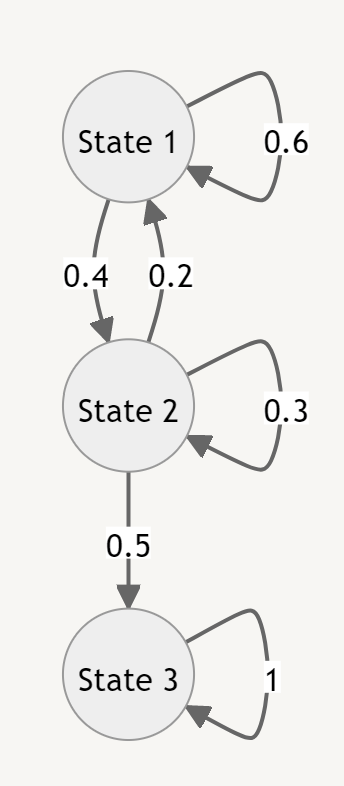
\includegraphics[width=2.0cm]
                      {Images/Figures/states transition figure.png}
                 \caption{図の説明}
                 \label{ラベル名}
                \end{figure}
            \end{column}
        \end{columns}        
    \end{exampleblock}
\end{frame}


\subsection{Lemmas}
\begin{frame}
    \begin{lemma}
        \label{lemmaA} The product of two stochastic matrices is another stochastic matrix.        
    \end{lemma}  
    Proof.\\
    let $P=(p_{ij}) _{ij}, Q = (q_{ij}) _{ij}$ be stochastic matrices. From definition of matrix product, $(PQ)_{ij} = \sum_{k} p_{ik}q_{kj}$ . 
    Also, stochastic matrices satisfies 
    $\forall i\in\mathbb{N},\quad\sum_{j}  p_{ij} = 1,\quad\sum_{j}  q_{ij} = 1$ 
    \[
    \therefore \sum_{j} (PQ)_{ij}
    = \sum_{j} \sum_{k} p_{ik}q_{kj}
    = \sum_{k} \left(p_{ik}\sum_{j}  q_{kj}\right) = \sum_{k} p_{ik} = 1
    \]
    Therefore, sum of  $i$th row of $PQ$ equals to 1, thus $PQ$ is another stochastic matrix.\qed
\end{frame}

\begin{frame}
    \begin{lemma}
        \label{lemmaB} Every eigenvalue $\lambda$ satisfies 
        $|\lambda|\le1$.
    \end{lemma}
    Proof. \\
        Let $P=(p_{ij}) _{ij}$ be stochastic matrices, $v = (v_i)_i$ be eigenvector of $P$, and $\lambda$ be eigenvalue.
        Also, define $m$ as below.
        $$
        m = \argmax_{i} \{|v_1|,...,|v_n|\} 
        $$
        Then, because $Pv = \lambda v$, 
        \[
        \sum_i p_{mi} v_i = \lambda v_m \\
        \therefore |\lambda |
        = \frac{|\sum_i p_{mi} v_i |}{|v_m|} 
        \le \frac{\sum_i p_{mi} |v_i|}{|v_m|}
        \le \frac{\sum_i p_{mi} |v_m|}{|v_m|}
        = \frac{1\cdot |v_m|}{|v_m|} = 1 \qed
        \]
\end{frame}

\begin{frame}
    \begin{lemma}
        \label{lemmaC} Every stochastic matrix has at least one eigenvalue equal to 1.
    \end{lemma}  
    Proof.\\
    Let $P=(p_{ij}) _{ij}$ be a stochastic matrix, $v_0$ be a vector s.t.$ v_0 = (1,\cdots,1)$, then
    \[
    \forall i, (Pv_0)_i = \sum_j p_{ij} = 1 = (v_0)_i
    \therefore Pv_0 = v_0
    \]
    Thus, $P$ has at least one eigenvalue equal to 1. \qed
\end{frame}
% % Remember to input this to the presentative tex file before compiling.
\section{Introduction to further theory of Markov processes}
\begin{frame}{What we will learn next}
    \begin{enumerate}
        \item \textbf{Discrete} State-space -> \textbf{Continuous} state-space
        \begin{enumerate}
            \item ex) Processes with Gaussian Noise like AR(1):
            \[
            Z_{t+1} = \alpha Z_t + \varepsilon_t, 
            \quad t=0,1,...,\quad \varepsilon \sim N(0,\sigma^2)
            \]
        \end{enumerate}
        \item \textbf{Dicrete} time -> \textbf{Continuous} time
        \begin{enumerate}
            \item ex) Random Walk -> Brownian Motion
        \end{enumerate}
    \end{enumerate}
    \uncover<1->{\Large I will introduce further theories at next b-seminar!}
\end{frame}
\section{Summing Up}

% This section is a placeholder for you to go over crucial points to takeaway from your presentation.

\begin{frame}
\begin{center}
\Huge Thank You!
\end{center}
\end{frame}

% Bibliography/References
\begin{frame}[allowframebreaks]
	\frametitle{References}
	\nocite{*}
	\printbibliography
\end{frame}

% Appendix
% \appendix
% % The appendix tex file gets inputted after the /appendix command in the main tex file.
% Treat your appendices as you would regular chapters, sections and subsections, and they would be automatically discounted as appendices.

\section{Appendix I} \label{app1}
%\subsection{Appendix 1.1 Scenario 1}
%\subsection{Appendix 1.2 Scenario 2}
\begin{frame}
    \begin{remark}
    This is what an appendix would look like.
    \end{remark}
    \begin{exampleblock}{Example}
    {\gray \lipsum[2][1-20]}
    \end{exampleblock}
\end{frame}

\section{Appendix II} \label{app2}
\begin{frame}
    \begin{block}{Relevant Title}
    {\gray \lipsum[2][1]}
    \end{block}
    \begin{exampleblock}{Example of Appendix II}
    {\gray \lipsum[4][1-20]}
    \end{exampleblock}
\end{frame}

\end{document}